\documentclass{article}
\usepackage{graphicx} % Required for inserting images
\usepackage{amsmath}
 \usepackage{float}
 \usepackage{url}
 \usepackage{subcaption}
\usepackage{bm} % in preamble
\newcommand{\norm}[1]{\lVert #1 \rVert}
\renewcommand{\vec}[1]{\bm{#1}}
\title{Two Class Support Vector Machines}
\author{Arnav Yadnopavit}
\date{August 2025}

\begin{document}

\maketitle

\section{Introduction}
Support Vector Machine (SVM) is a powerful supervised machine learning algorithm primarily used for classification and regression tasks. It works by finding the optimal hyperplane that best separates data points into different classes.


\section{Working}
We have data points $\vec{x_i}$ of dimension $n$ which have their specific labels $y_i$ (As in categories).\\

The end goal is to find a hyperplane $\vec{wx^\top+b=0}$ which gives the maximum distance from all the points. This is called a maximum margin classifier.

\begin{align*}
    y_i&(\vec{w}^\top \vec{x_i} +b)\ge 1\\
    Margin&=\frac{2}{\norm{\vec{w}}}\\
    min&\frac{\norm{\vec{w}}^2}{2} , y_i(\vec{w}^\top\vec{x_i}+b)\ge 1
\end{align*}
To minimise, over the given constraints we need hinge loss.\\
Hinge loss basically penalises points that lie on the wrong side of the hyperplane wrt the labels.\\
It can be written as:
\begin{align*}
    HingeLoss(\vec{w},b,\vec{x_i},y_i)=max(0,1-y_i(\vec{w}^\top\vec{x_i}+b))
\end{align*}
Thus calculating hinge loss gradient expression\\
Let $f_i(\vec{w},b)=y_i(\vec{w}^\top\vec{x_i}+b)$,Then\\
If $f_i\ge1$
\begin{align*}
    \nabla w=0, \nabla b=0
\end{align*}
else
\begin{align*}
    \nabla w=-h(\vec{w}-y_i\vec{x_i}), \nabla b=hy_i\vec{x_i}
\end{align*}

\section{Results}
\begin{figure}[H]
    \centering
    \begin{subfigure}{0.5\textwidth}
        \centering
        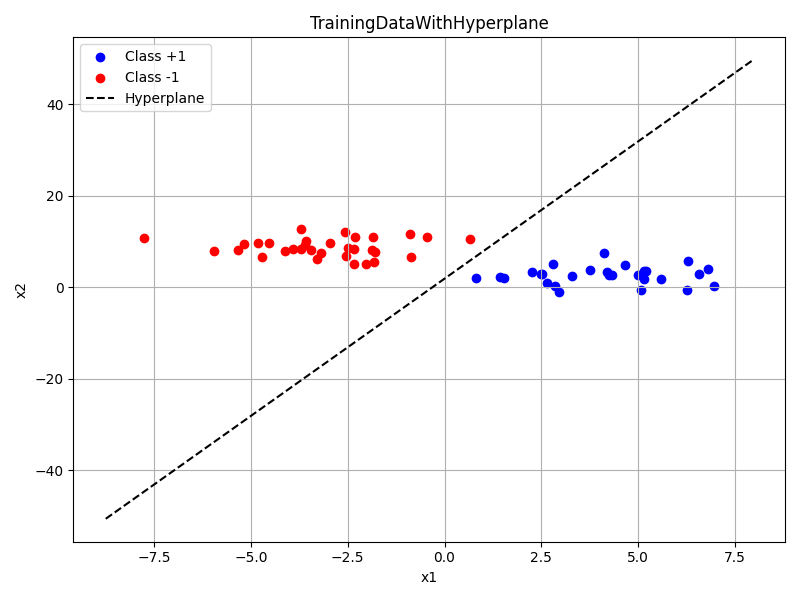
\includegraphics[height=4cm]{figs/TrainingDataWithHyperplane.png}
    \end{subfigure}%
    \begin{subfigure}{0.5\textwidth}
        \centering
        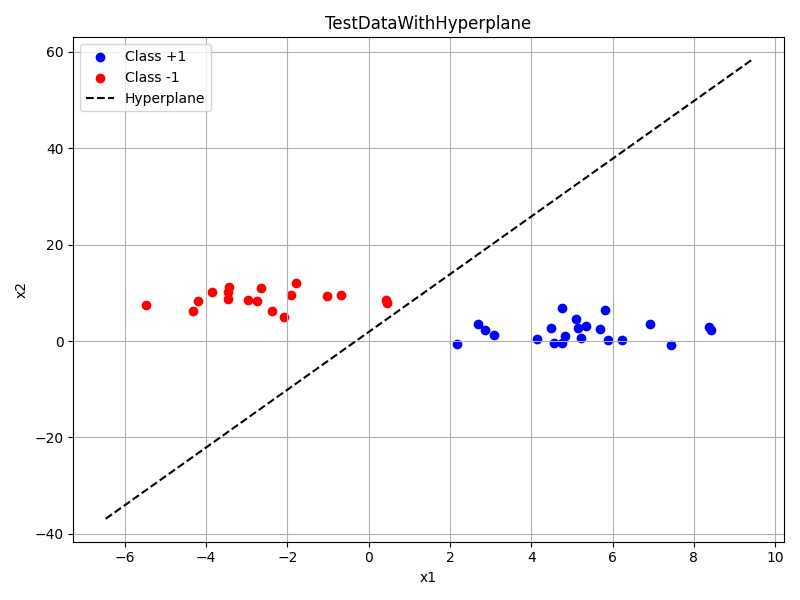
\includegraphics[height=4cm]{figs/TestDataWithHyperplane.png}
    \end{subfigure}
\end{figure}

\section{Conclusion}

Linear Two-Class Soft-Margined SVM successfully applied.Check out the following url for codes,plots,and a real data application \\
\url{https://github.com/ArnavYadnopavit/CoolStuff/tree/main/SVM}\\
\\\\

\centering{Thank you!}







\end{document}

